\documentclass[a4paper,12pt]{IEEEtran}
\usepackage{graphicx}
\graphicspath{{./report_plots/}}
\begin{document}

\title{CSC 510 Assignment 3 Report}
\author{Justin Oakley}
\maketitle\

\pagenumbering{arabic}
\tableofcontents
\newpage

\section{Introduction}
This report is about building an understanding of how big data systems function and process big data in a manner suitable for machine learning. The reason why these big data systems are important in the field of data science is due to the continuous evolution of big data systems and resources, so having a fundamental understanding of current systems will assist in the development of this knowledge. There are two main ways of implementing a big data system for big data analysis and machine learning: on a local machine or on a cloud platform, such as Microsoft Azure, Amazon Web Services, or Google Cloud Platform. As for the type of systems utilized in big data science, the Hadoop clusters and Spark clusters are two of the most popular and widely used technologies for data handling and machine learning.

In this assignment, Apache Spark 2.4.0 on an Apache Hadoop cluster will be the type of big data system utilized for machine learning. As for the data that will be processed for machine learning, two network traffic-type datasets, called \textit{nslkdd-version1.csv} and \textit{nslkdd-version2.csv}, were selected. Using these datasets and this big data system, Spark's version of Decision Tree classification was performed for the actual machine learning process to create and refine a model to produce high-quality classification results and to be used for predicting accurate category labels. It should be noted that all coding for the experiment is done in a Jupyter Notebook using the Python 3 language.

\section{Machine Learning on the Apache Spark Big Data System}
\subsection{Procedure}
The first step taken in setting up Apache Spark for the data analyzation process of \textit{nslkdd-version1.csv} and \textit{nslkdd-version2.csv} was to install the proper files need for a standalone Spark cluster to be run on an Ubuntu Linux virtual machine and then perform the setup of the environment. Once this is done, the master server and slave servers were launched to make the Spark cluster ready for data handling. Now that the big data system was fully functional, an iPython Notebook was created, all the appropriate libraries were imported for the application (including a library called "findspark" which integrates the Jupyter environment with Spark), and a SparkContext was initialized. Following these important steps, the data preprocessing and machine learning was able to be executed.

Since both datasets were known to be of the same source, yet each set had major differences from each other, preprocessing was mandatory prior to classification, especially because there were only two types of network-traffic that were going to be analyzed: normal-traffic and attack-traffic. With this in mind, the data was read in and any observations that had null values for any of the features, if any had null values, were dropped. Now, it was known that the \textit{nslkdd-version2.csv} columns were a subset of the features of \textit{nslkdd-version1.csv}, so only the intersection of both sets' columns were utilized in the supervised learning. Following this, the label column of \textit{nslkdd-version1.csv} was converted from categorical data to indexed, numerical data; then each observation in both datasets were labeled (using only zeros and ones) either as normal-traffic or attack-traffic. Following that, the original label columns were dropped since they were no longer needed for classification.

For obtaining accurate data, a set's columns were statistically compared to the other set's counterpart columns, respectively, and any features with matching stats were kept while features with non-matching stats were dropped because they could not be deemed reliable. Once this was finished, it was recognized that some of the columns that were kept contained a vast amount of zero-values; so it was decided that any columns that had a third-quartile statistic that was zero should be dropped. Finally, the data features were assembled into vectors and standarized. At this point, the data was now primed and ready for Decision Tree classification.

Using Spark's version of a Decision Tree classifier, the data was split into training and testing and both sets were used to fit and transform the model; because the technique used in the experiment was a Decision Tree, probabilistic quantitative measures were used to train the data and qualitative measures were used to test and validate the data. Once the \textit{nslkdd-version1.csv} and \textit{nslkdd-version2.csv} Decision Tree models were trained and tested, they were then evaluated by the Binary-Classification Evaluator and the areas under the Receiver Operating Characteristic Curve were derived from the evaluation. Finally, the training and testing sets from both datasets are operated on by a tenfold cross validator to improve the model to work proficiently on unseen data. Now that the classification process has finished, the Decision Tree models and their results can now undergo data analyzation to determine its effectiveness.

\subsection{Analyzation of Machine Learning Results}
As a result of the cleaning of the data, the preprocessing techniques of the \textit{nslkdd-version1.csv} and \textit{nslkdd-version2.csv} sets can be deemed as effective since all of the machine learning results for both sets are equivalent to each other, respectively. Because of this, both Decision Tree models and sets of predictions will be referred to as a singular model and singular set from here on out.

According to the Binary-Classification evaluation of the "nslkdd" Decision Tree, the area under the ROC curve was calculated to be within a range of 0.93 and 0.95, depending on what observations were sampled from the original source set. This can be seen in the following visualization:
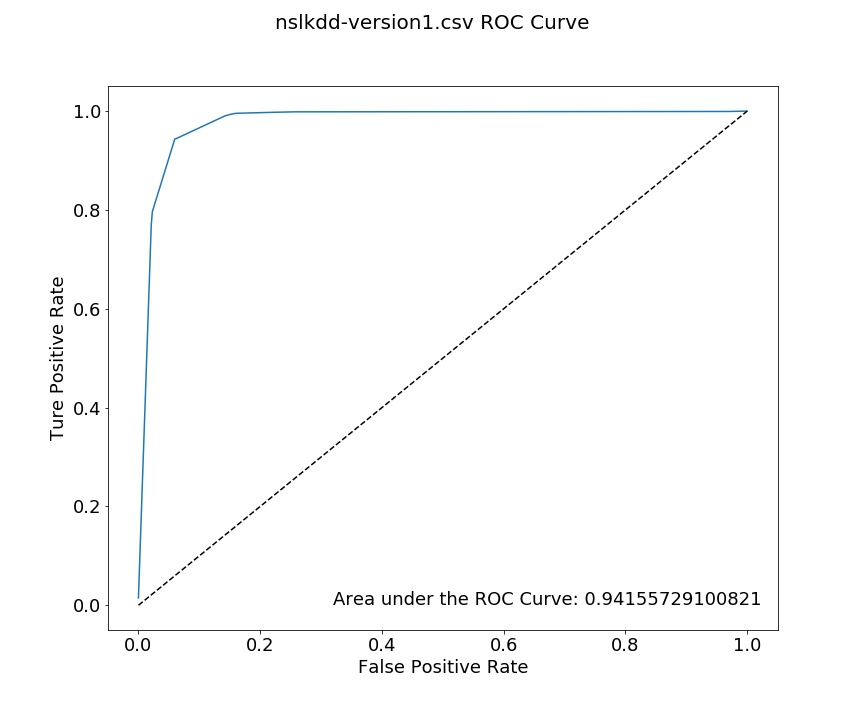
\includegraphics[width=8cm]{v1_roc}

The area under the ROC curve is important in binary-classification because it is used as a metric for computing the probability of each class and constructing a prediction threshold; the area under the ROC curve is also utilized for finding the sensitivity of the false-alarm rate. Since the sensitivity for detecting a false-alarm is over 90\%, then it is simple to determine that the false negative rate is lower than 10\%. Also by observing the ROC plot, it can be noticed that the curve is close to the upper left corner of the graph and infers that specificity is slightly less than 1, meaning that the classification lacks false positives.

As for the tenfold Cross-Validator that was also run on the training and testing sets, its accuracy score was computed to be within a range of 0.97 and 0.98, once again depending on the observations randomly selected from the sample. With two types of accuracy-scores (one being the Binary-Classification evaluation and the other being the Cross-Validation) being higher than 90-percent, it can be inferred that the Decision Tree classifier model built on the traffic-type dataset is accurate in predicting if a network traffic observation is a normal-type or a attack-type.

Now that the classification model can seen as highly-accurate, the question of the model's most important features can be resolved. According to Spark's tools for data analysis, only four of the preprocessed features used in classification had an importance-value higher than 0.05 (as seen in the following figure), with the most significant feature importance being over 0.60.
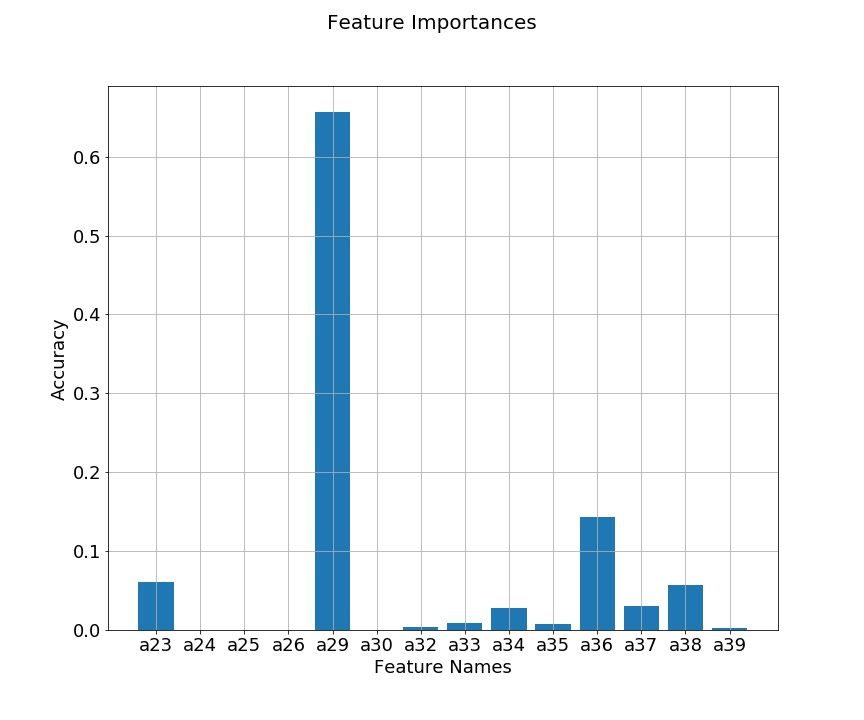
\includegraphics[width=8cm]{v1_feature_importances}

With all of this information in mind, the last step in analyzing the machine learning results is to compare both the number amount of predicted labels with the acutal number of predicted labels. As seen in the following pie-chart, the ratio between normal-types and attack-types for the original test set labels demonstrates an almost even split among the labels.
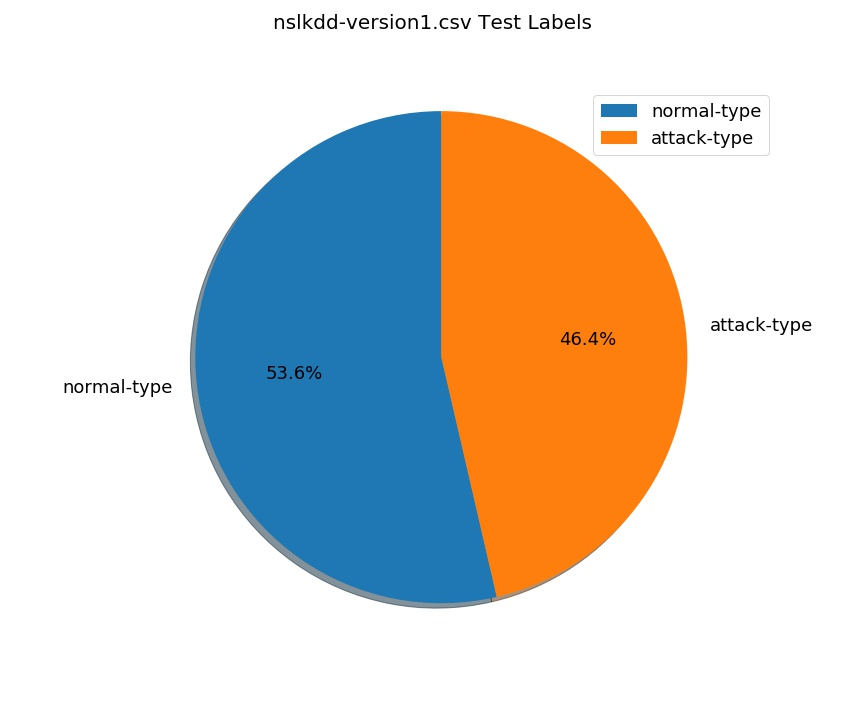
\includegraphics[width=8cm]{v1_test_pie}

Compared to the ratio of network traffic-types derived from the predicted set, the numbers of both ratios are not equivalent, but are approximately close to each other in value.

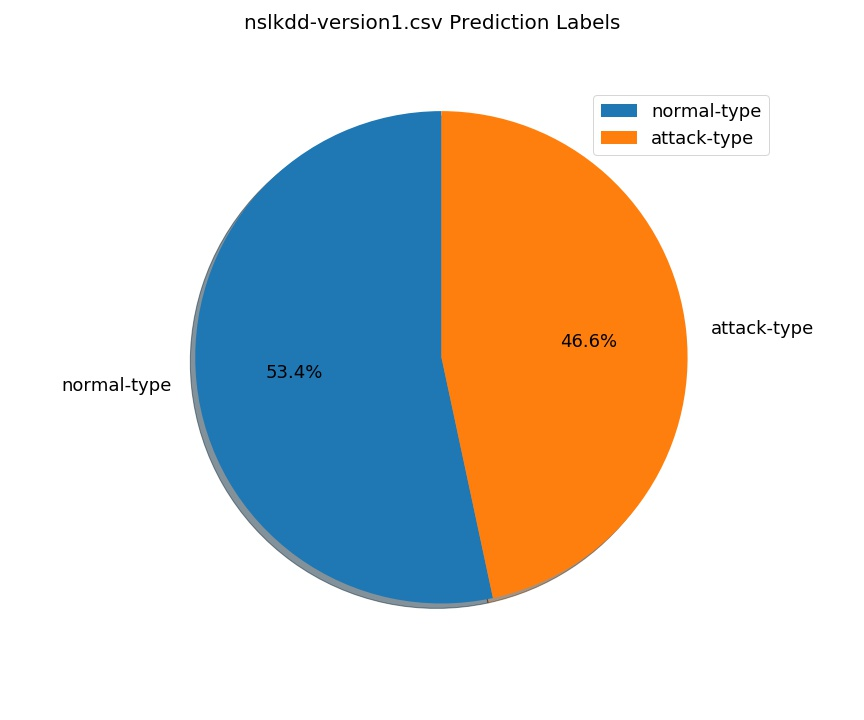
\includegraphics[width=8cm]{v1_pred_pie}

This is not surprising since both the AUC and the tenfold Cross-Validation accuracy-score are greater than 0.90. With this in mind, it can be concluded that the machine learning process was efficient and Decision Tree classification lead to acceptable results for prediction for the network traffic-type dataset.

\section{Spark's Decision Tree Classification Review}
In conclusion, the assignment was successful in developing an understanding of the functionality of a big data system such as Apache Spark on a Hadoop cluster and comprehending the power that goes into this type of big data technology. Working with the tools provided by the Spark computational engine allowed for good insight on how on to navigate and use a big data system such as this. The experiment was also effective in showing the impact of the preprocessing of data for machine learning and computational prediction. With this knowledge and experience, a further appreciation and understanding of big data science and machine learning can be developed as well as a fundamental and working comprehension of big data systems, their abilities and attributies, and their continuous evolution.

\end{document}